\documentclass[12pt,letterpaper]{report}
\usepackage[margin=1in]{geometry}
\usepackage{titlesec}
\usepackage{amsmath}
\usepackage{amssymb}
\usepackage[colorlinks=true,urlcolor=black,linkcolor=black]{hyperref}
\usepackage{graphicx}
\usepackage{textcomp}
\graphicspath{ {./images/} }
% extra packages you need

\titleformat{\chapter}{\bf\huge}{\thechapter}{20pt}{\huge\vspace{-.5em}}

\begin{document}

\title{\begin{figure}[htb]
\begin{center}

\includegraphics[width=8cm]{univ_logo}
\end{center}
\end{figure}SOEN 6011 : SOFTWARE ENGINEERING PROCESSES\\[.5em]
SUMMER 2022\\\vspace*{0.9in}
\begin{Large}
\textbf{ETERNITY} 
\end{Large}
\vspace*{0.9in}
\begin{Large}
\textbf{\\PROBLEM - 1} 
\\Function Description 
\end{Large}}
\author{By Prathika Anup Suvarna (40156790)}
\maketitle 
\pagenumbering{roman}
\setcounter{page}{0}

\tableofcontents

% delete this section if no figures
\listoffigures\addcontentsline{toc}{chapter}{List of Figures}
% This will automatically be populated if you included figures in your report.


%%%%%%%%%%%%%%%%%%%%%%%%%%%%%%
\chapter{Function Description}
\pagenumbering{arabic}

\normalsize{The function Standard Deviation, $\sigma$ is the measure of how far each observed value is from the mean, and it has the following formula: \cite{definition} 
$$SD, \sigma = \sqrt{\frac{1}{N}\sum_{i=1}^{N}(x_i-\mu)^2}$$
where,\\$\sigma =$ Population standard deviation\\
N = Number of observations in population\\
$x_i = i^{th}$ observation in the population\\
$\mu =$ Population mean}

\begin{figure}[h]
 \centering
 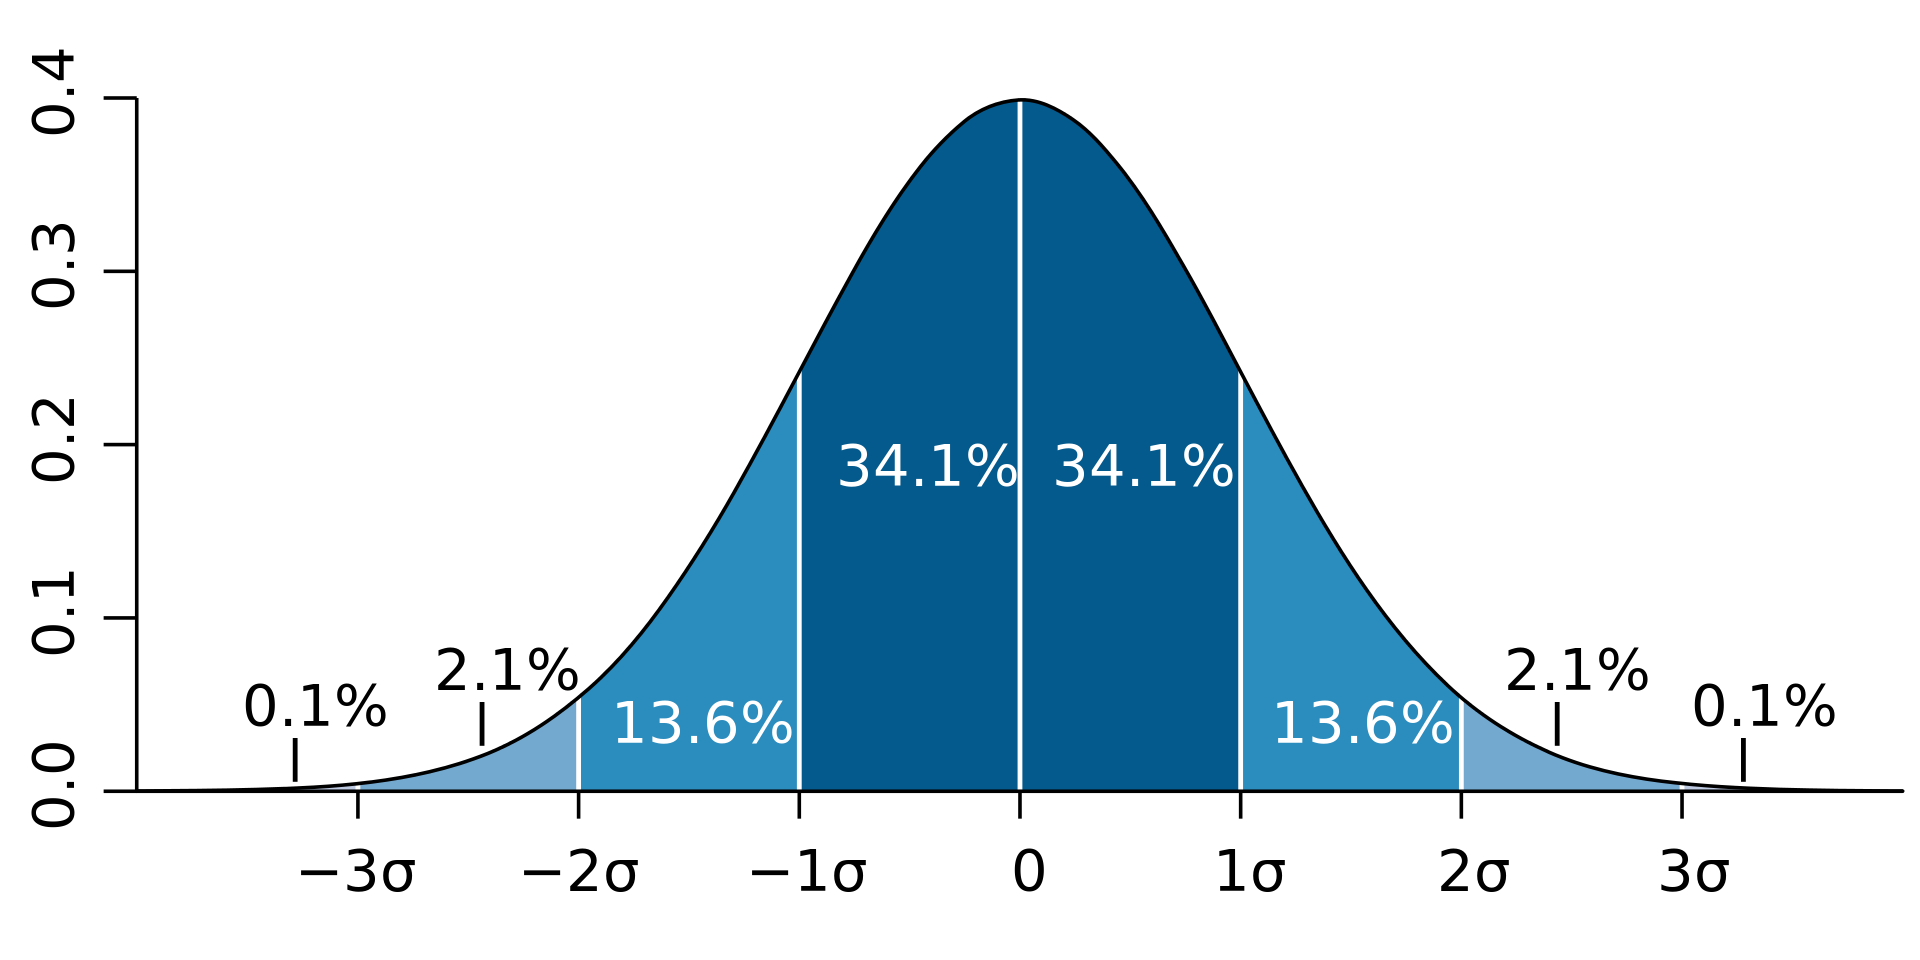
\includegraphics[width= 6cm]{images/Standarddev.png}
  \caption{A Bell Curve is used to represent SD.}\cite{definition}
\end{figure}

\normalsize{The above graph of a normal distribution represents data in real life. The mean, $\mu$ is in the center and each segment (colored in dark blue to light blue) represents one standard deviation away from the mean i.e. $2\sigma$ means two standard deviations from the mean.\cite{Graph}
\\\\
\textbf{Domain:}\\
The domain of Standard Deviation, $\sigma$ is $\mathbb{R}$, i.e. (-$\infty$, +$\infty$). Since the function takes a range of x values, the positive values of $x$ trend toward +$\infty$, negative values of $x$ trend toward -$\infty$, and if all values in the array is 0 then it outputs 0. 
\\
\\\textbf{Co-Domain:}\\
The co-domain of Standard Deviation, $\sigma$ is positive $\mathbb{R}$, i.e. (0, +$\infty$). Since the function is square root of variance, which is the average squared deviation from the mean, it can never be negative.\cite{negativevalues}
\\
\\\textbf{Characteristics that make it unique:}
\begin{itemize}
  \item 	Standard deviation is only used to measure dispersion around the mean of a data set.
  \item  	Standard deviation is never negative. 
  \item 	For data with approximately the same mean, the greater the spread, the greater the standard deviation
  \item     If all data set values are same, the standard deviation is zero as each value is equal to the mean. 
\end{itemize}}

{\let\clearpage\relax \chapter{Context of Use}}
 
The users of the calculator shall be using it to calculate the result of the standard deviation function on an array of input numbers. This array shall have positive numbers, negative numbers and decimals and must have atleast two numbers in it. The calculator shall allow the user to enter numbers using \textit{0-9} keys, the decimal point and the minus key for negative values. The user shall click on the standard deviation button in order to generate and view the result for the input given. The calculator should return the result or a message that indicates why it was unable to do so.

\begin{figure}[h]
 \centering
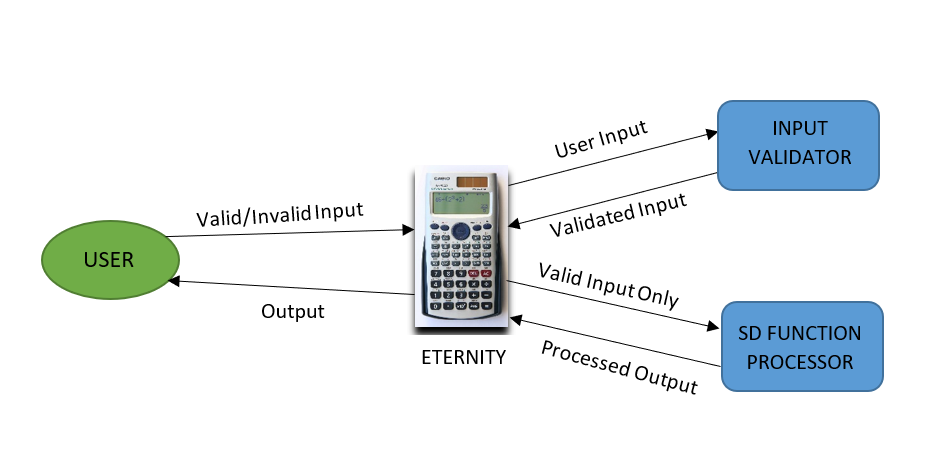
\includegraphics[width=15cm]{contextuse}
  \caption{Input/Output Flow of ETERNITY.}
\end{figure}




%%%%%%%%%%%%%%%%%%%%%%%%%%%%%%
\begin{thebibliography}{9}
    \addcontentsline{toc}{chapter}{Bibliography}

    % delete all of these example references, and replace them with references for your report.
    \bibitem{definition} 
    Wikipedia: 
    \textit{Standard Deviation},
    \texttt{https://en.wikipedia.org/wiki/Standard\_deviation/}
   
   \bibitem{Graph}
    StatisticsHowTo:
    \textit{What does SD look on a graph?},
    \texttt{https://www.statisticshowto.com/probability\-and\-statistics/standard\-deviation/}

    \bibitem{negativevalues}
    Macroption: 
    \textit{Why Standard Deviation can't be nagative?},  
    \texttt{https://www.macroption.com/can-standard-deviation-be-negative/}
    
 
    
\end{thebibliography}



\end{document}